\documentclass{beamer}
\usetheme{Frankfurt}
\setbeamertemplate{footline}[frame number]
\setbeamercovered{transparent}
\usepackage{graphicx,animate,tikz,amsmath}
\graphicspath{{../images/},{../images/movie_por0_stre6/},{../images/movie_por50_stre6/},{../images/movie_por50_stre3/},{../images/movie_por50_stre3_ang45/}}


\AtBeginSection[]{
	\begin{frame}
	\vfill
	\centering
	\begin{beamercolorbox}[sep=8pt,center,shadow=true,rounded=true]{title}
		\usebeamerfont{title}\insertsectionhead\par%
	\end{beamercolorbox}
	\vfill
\end{frame}
}

\title{SPH simulations for planetary defense}
\author{Maximilian Rutz}

\begin{document}

\begin{frame}[plain]
	\maketitle
\end{frame}

\begin{frame}[plain]{Roadmap}
	\tableofcontents
\end{frame}

\section{Dart and Hera missions}
\begin{frame}
	\begin{tikzpicture}[remember picture,overlay]
		\node[at=(current page.center)] {
			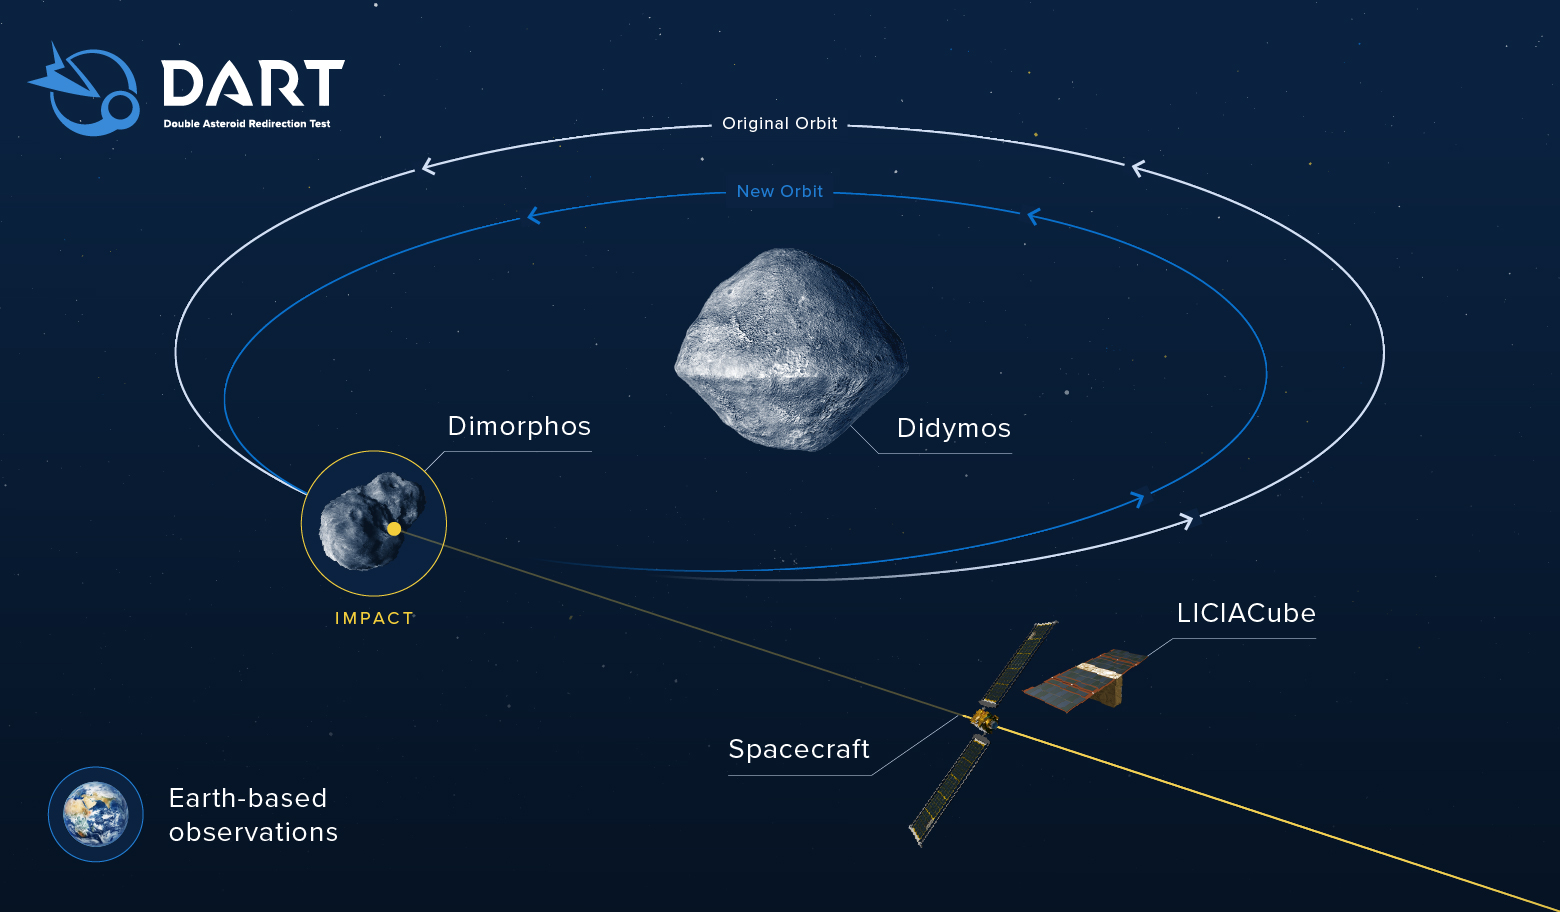
\includegraphics[keepaspectratio,
				width=\paperwidth,
				height=\paperheight]{dart_mission.jpg}};
	\end{tikzpicture}
\end{frame}

\begin{frame}{Dart Mission}
	%https://dart.jhuapl.edu/Gallery/media/graphics/lg/DART-infographic_v4.jpg
	\begin{itemize}[<+->]
		\item Launch in July 2021 on a SpaceX Falcon 9
		\item Impact in fall 2022
		\item Impact at ~0.04 au to Earth, ~15x Earth-Moon, ~1/10x Earth-Mars
		\item Observations with LICIACube and earth based telescopes
	\end{itemize}
\end{frame}

\begin{frame}{Hera Mission}
	\begin{tikzpicture}[remember picture,overlay]
		\node[at=(current page.center)] {
			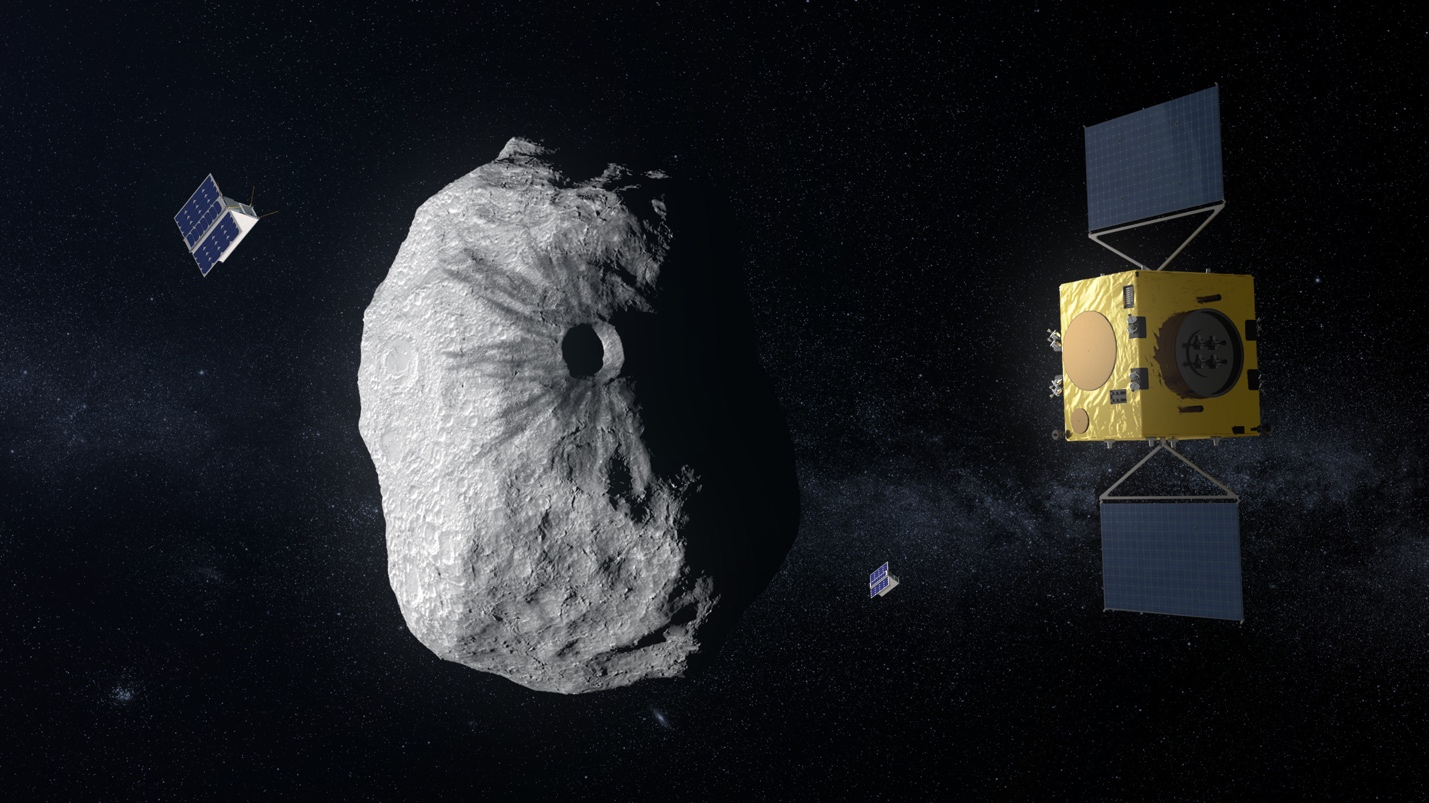
\includegraphics[keepaspectratio,
				width=\paperwidth,
				height=\paperheight]{hera_mission.jpg}};
	\end{tikzpicture}
\end{frame}

\begin{frame}{Hera Mission}
	%https://www.esa.int/var/esa/storage/images/esa_multimedia/images/2018/06/testing_deflection/1%5359917-7-eng-GB/Testing_deflection_pillars.jpg
	\begin{itemize}[<+->]
		\item Launch in 2024
		\item Arrival in 2026
		\item Detailed images and measurements
	\end{itemize}
\end{frame}

\begin{frame}
	\begin{tikzpicture}[remember picture,overlay]
		\node[at=(current page.center)] {
			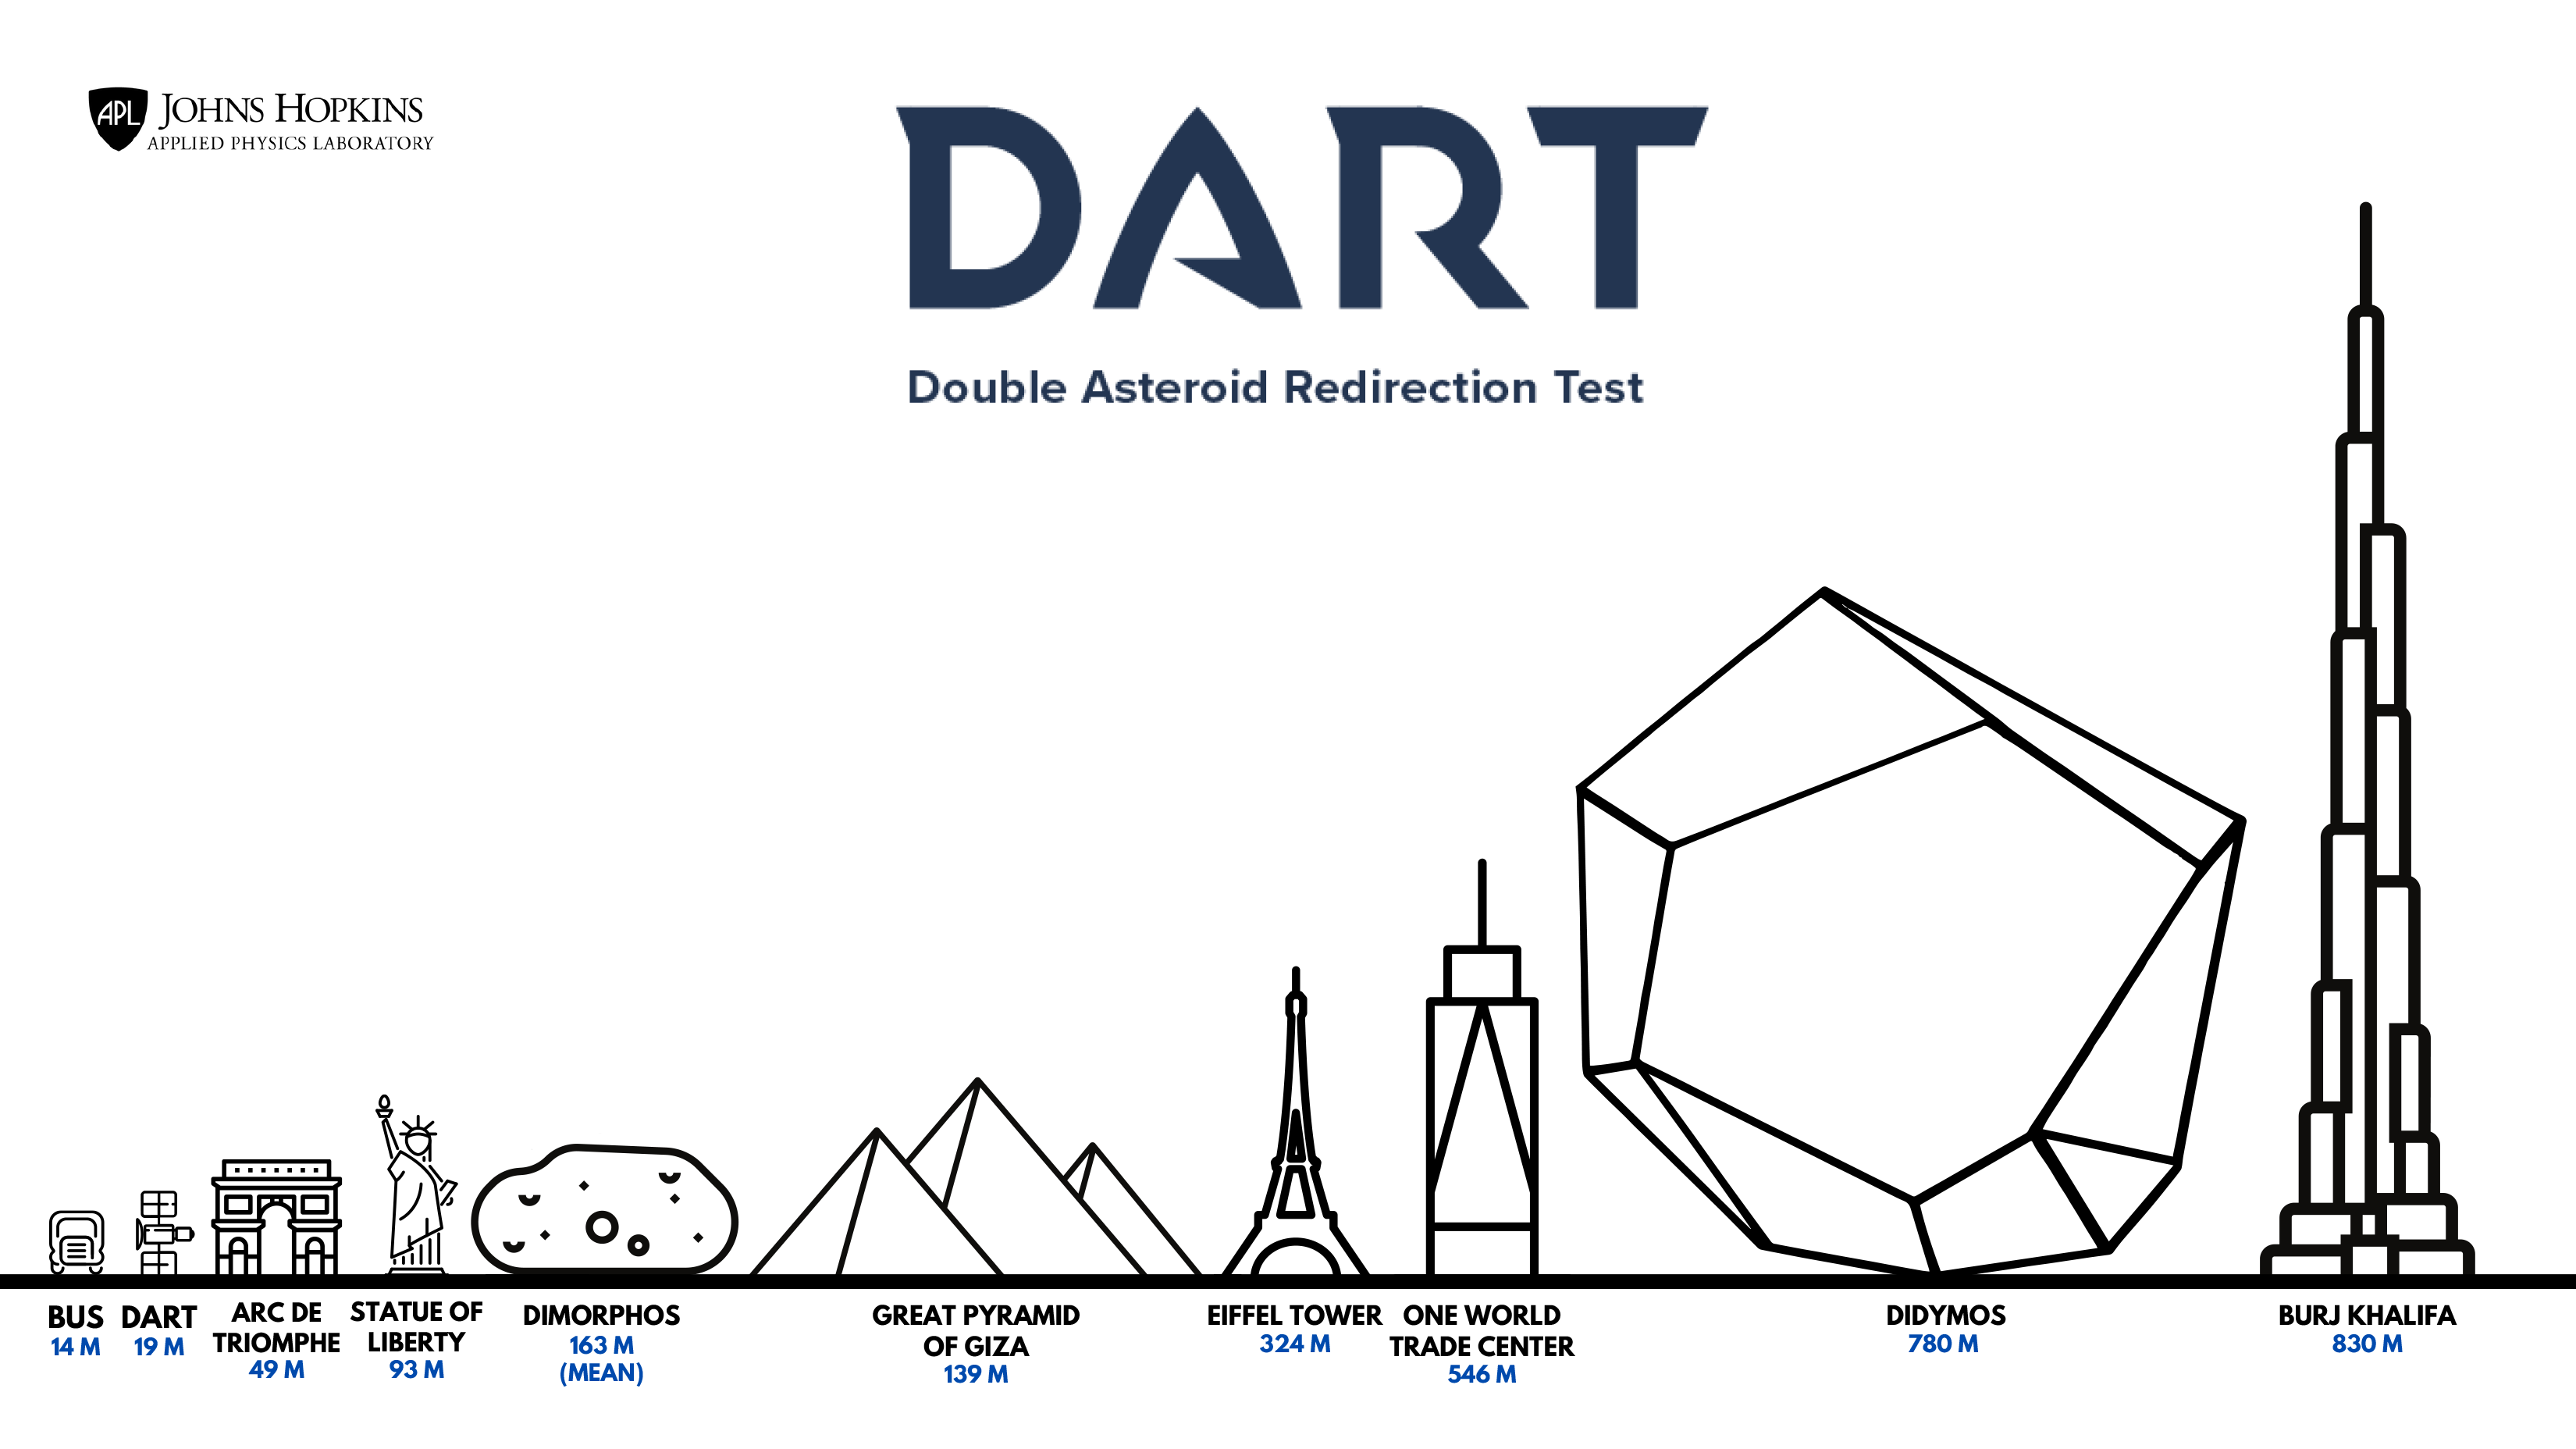
\includegraphics[keepaspectratio,
				width=\paperwidth,
				height=\paperheight]{asteroids_size.png}};
	\end{tikzpicture}
\end{frame}

\section{SPH setup}
\begin{frame}{Simulation goals}
	Compare numerical results with observations to:
	\begin{enumerate}[<+->]
		\item Test numerical codes
		\item Identify target properties through parameter studies
	\end{enumerate}
\end{frame}

\begin{frame}{Simulation scenario}
	Target:
	\begin{itemize}[<+->]
		\item 160 meter diameter
		\item Important parameters such as porosity and strength unknown
	\end{itemize}
	Impactor:
	\begin{itemize}[<+->]
		\item 500 kg mass
		\item 6 km/s impact velocity
		\item Main body 1.3 x 1.2 x 1.2 meter
	\end{itemize}
\end{frame}

\begin{frame}{Smoothed Particle Hydrodynamics}
	\begin{columns}
		\begin{column}{0.55\textwidth}
			\begin{itemize}[<+->]
				\item Gridfree method
				\item Particles move through space with a velocity
				\item Particles carry physical quantities like density, pressure or energy
				\item Hydrodynamic/ continuum mechanics equations are solved for every particle
			\end{itemize}
		\end{column}
		\begin{column}{0.4\textwidth}
			\vspace{\topsep}
			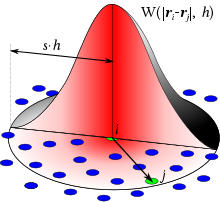
\includegraphics[width=\columnwidth]{sph_method.png}
		\end{column}
	\end{columns}
\end{frame}

\begin{frame}{Miluphcuda solid models}
	\begin{itemize}[<+->]
		\item Pressure dependent strength model
		\item Fragmentation for brittle materials
		\item p-$\alpha$ porosity model
		\item Tillotson equation of state
	\end{itemize}
\end{frame}

\begin{frame}{Initial conditions}
	\begin{tikzpicture}[remember picture,overlay]
		\node[xshift=0cm,yshift=4.45cm] at (current page.south) {
			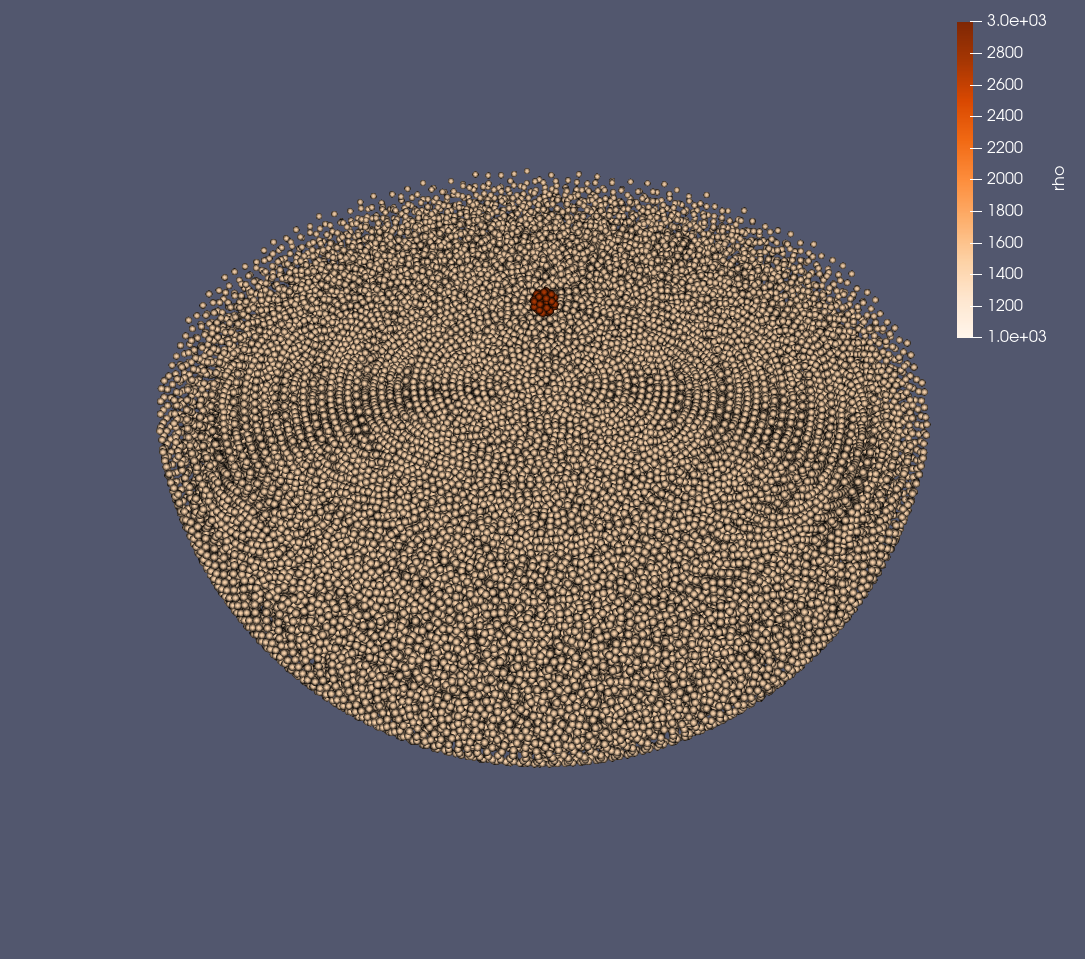
\includegraphics[keepaspectratio,
				width=\paperwidth,
				height=0.78\paperheight]{impact_start.png}};
	\end{tikzpicture}
\end{frame}
\begin{frame}{Initial conditions}
	\begin{tikzpicture}[remember picture,overlay]
		\node[xshift=0cm,yshift=4.45cm] at (current page.south) {
			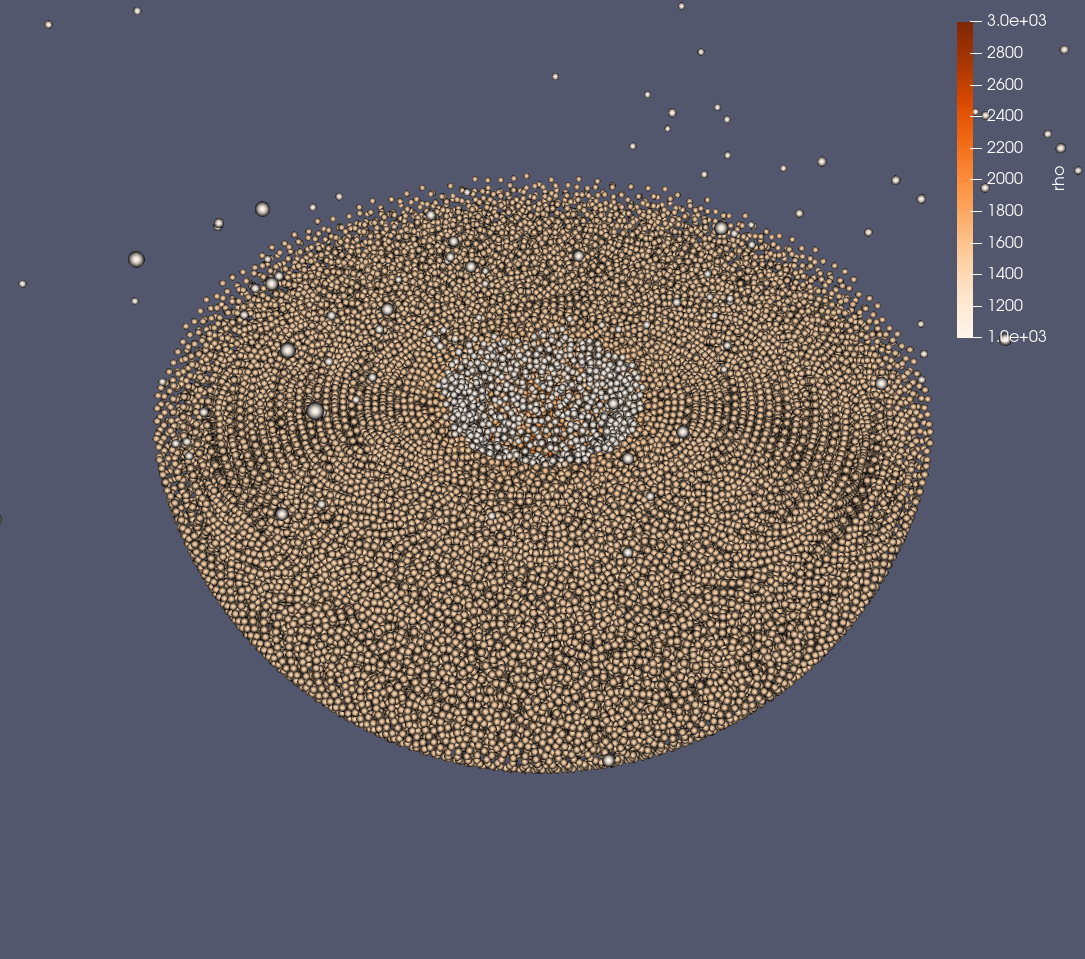
\includegraphics[keepaspectratio,
				width=\paperwidth,
				height=0.78\paperheight]{impact_end.png}};
	\end{tikzpicture}
\end{frame}

\begin{frame}{Initial conditions}
	Target:
	\begin{itemize}[<+->]
		\item Basalt
		\item 20 meter diameter halfsphere
	\end{itemize}
	Impactor:
	\begin{itemize}[<+->]
		\item Aluminum
		\item 0.75 meter diameter sphere
		\item 6 km/s impact velocity
		\item 500 kg mass
	\end{itemize}
\end{frame}

\section{SPH results}

\begin{frame}
	\begin{columns}
		\begin{column}{0.59\textwidth}
			\centering
			0\% porous, $Y_0$ = 1 MPa
			\animategraphics[controls=play,width=\linewidth ext=.png type=png]{100}{movie_por0_stre6.}{0000}{0300}
		\end{column}
		\begin{column}{0.59\textwidth}
			\centering
			50\% porous, $Y_0$ = 1 MPa
			\animategraphics[controls=play,width=\linewidth ext=.png type=png]{100}{movie_por50_stre6.}{0000}{0300}
		\end{column}
	\end{columns}
\end{frame}

\begin{frame}
	\begin{columns}
		\begin{column}{0.59\textwidth}
			\centering
			50\% porous, $Y_0$ = 1 MPa
			\animategraphics[controls=play,width=\linewidth]{100}{movie_por50_stre6.}{0000}{0300}
		\end{column}
		\begin{column}{0.59\textwidth}
			\centering
			50\% porous, $Y_0$ = 1 kPa
			\animategraphics[controls=play,width=\linewidth]{100}{movie_por50_stre3.}{0000}{0300}
		\end{column}
	\end{columns}
\end{frame}

\begin{frame}
	\begin{columns}
		\begin{column}{0.59\textwidth}
			\centering
			50\% porous, $Y_0$ = 1 kPa
			\animategraphics[controls=play,width=\linewidth]{100}{movie_por50_stre3.}{0000}{0300}
		\end{column}
		\begin{column}{0.59\textwidth}
			\centering
			50\% porous, $Y_0$ = 1 kPa, 45 deg angle
			\animategraphics[controls=play,width=\linewidth]{100}{movie_por50_stre3_ang45.}{0000}{0300}
		\end{column}
	\end{columns}
\end{frame}


\begin{frame}{Beta factor}
	Momentum change because of ejecta: $\boldsymbol{\beta} = 1 + \frac{p_{ejecta}}{p_{impactor}}$\pause
	\vfill
	Particles considered ejecta:
	\begin{itemize}[<+->]
		\item 1 impactor diameter above surface
		\item Positive velocity in z direction
		\item Absolute velocity above gravitational escape velocity
	\end{itemize}
\end{frame}

\setbeamercovered{invisible}
\begin{frame}{Beta factor}
	\begin{tikzpicture}[remember picture,overlay]
		\node[xshift=-2.9cm,yshift=5.9cm] at (current page.south) {
			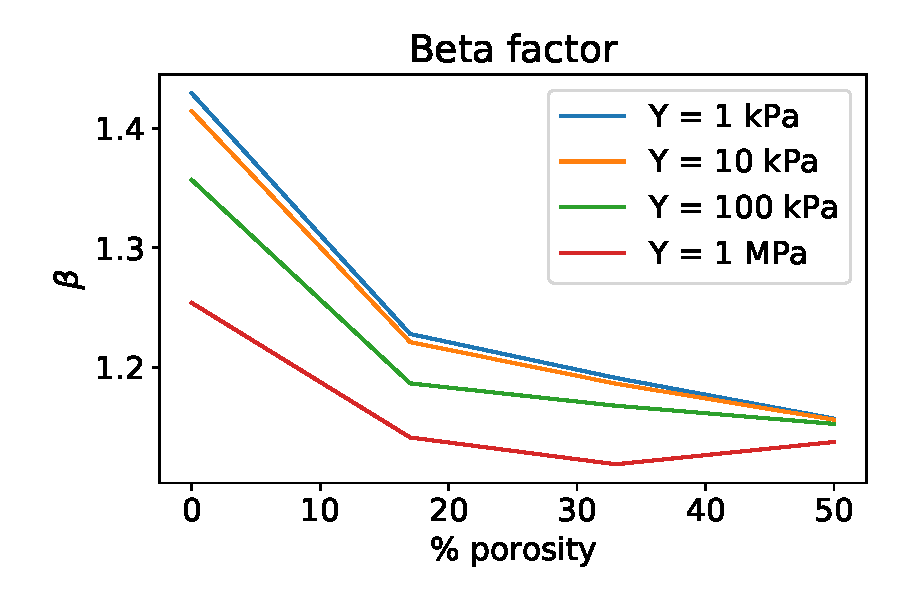
\includegraphics[keepaspectratio,
				width=\paperwidth,
				height=0.48\paperheight]{beta_results.pdf}};
	\end{tikzpicture}\pause
	\begin{tikzpicture}[remember picture,overlay]
		\node[xshift=0cm,yshift=1.8cm] at (current page.south) {
			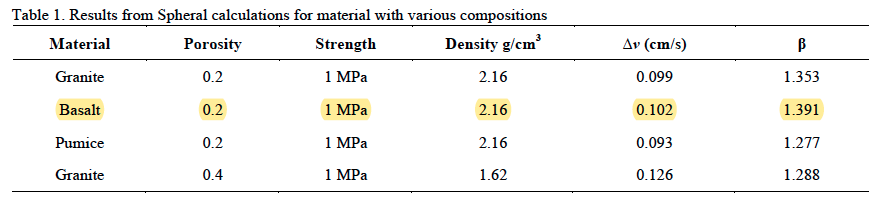
\includegraphics[keepaspectratio,
				width=0.98\paperwidth,
				height=\paperheight]{beta_stickle.png}};
	\end{tikzpicture}\pause
	\begin{tikzpicture}[remember picture,overlay]
		\node[xshift=3.5cm,yshift=5.8cm] at (current page.south) {
			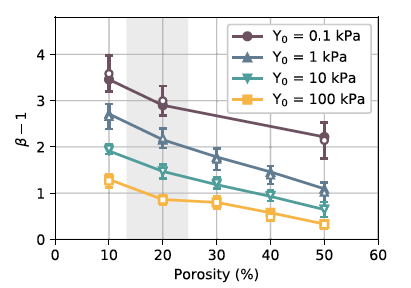
\includegraphics[keepaspectratio,
				width=\paperwidth,
				height=0.45\paperheight]{beta_raducan.png}};
	\end{tikzpicture}
\end{frame}

\begin{frame}{Crater shape}
	\begin{tikzpicture}[remember picture,overlay]
		\node[xshift=0cm,yshift=6cm] at (current page.south) {
			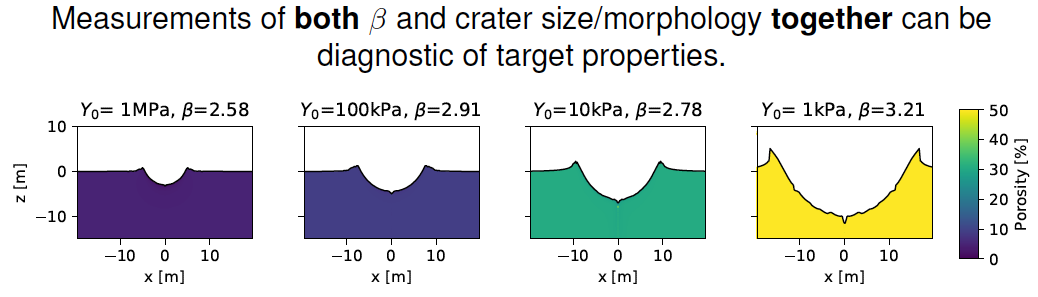
\includegraphics[keepaspectratio,
				width=0.9\paperwidth,
				height=\paperheight]{cratering_raducan_top.png}};
	\end{tikzpicture}
	\begin{tikzpicture}[remember picture,overlay]
		\node[xshift=-4.5cm,yshift=2.5cm] at (current page.south) {
			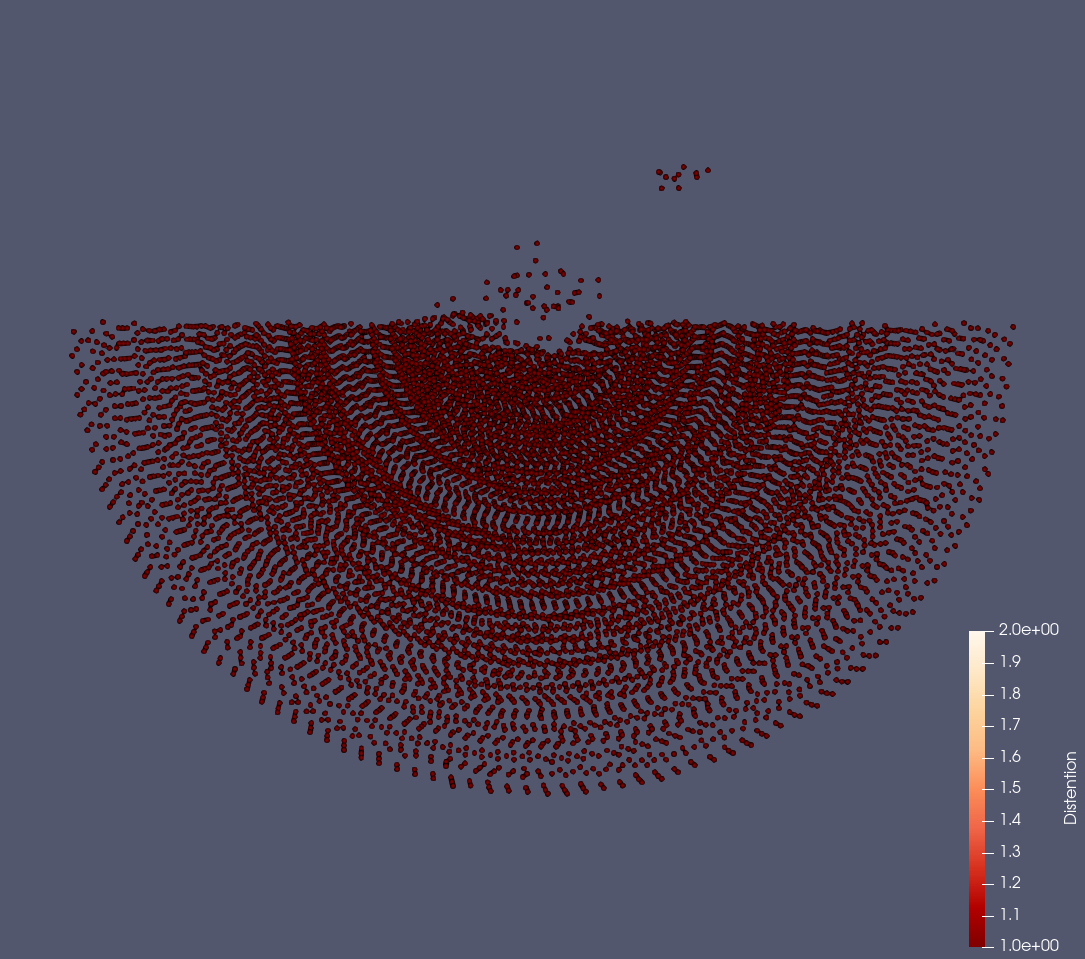
\includegraphics[keepaspectratio,
				width=0.25\paperwidth,
				height=\paperheight]{crater_por0_str1e6.png}};
	\end{tikzpicture}
	\begin{tikzpicture}[remember picture,overlay]
		\node[xshift=-1.5cm,yshift=2.5cm] at (current page.south) {
			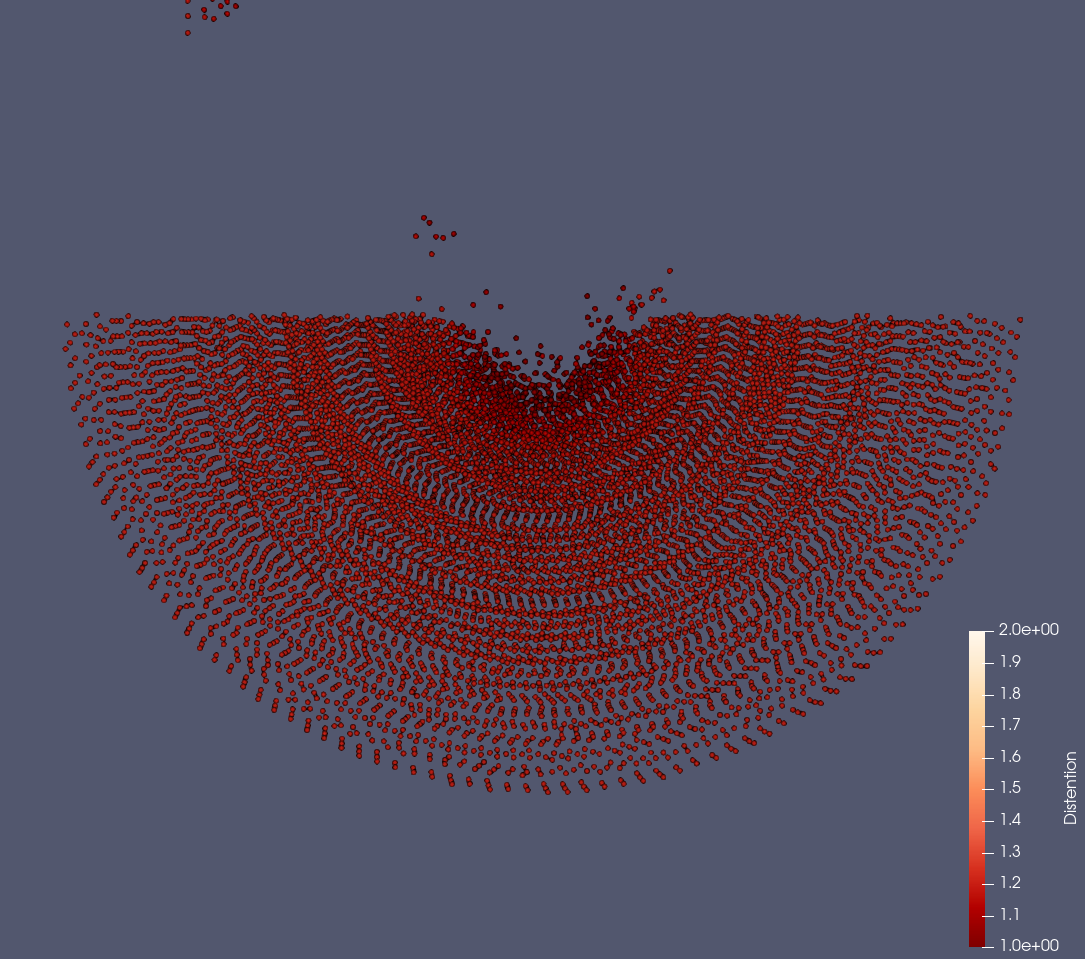
\includegraphics[keepaspectratio,
				width=0.25\paperwidth,
				height=\paperheight]{crater_por17_str1e5.png}};
	\end{tikzpicture}
	\begin{tikzpicture}[remember picture,overlay]
		\node[xshift=1.5cm,yshift=2.5cm] at (current page.south) {
			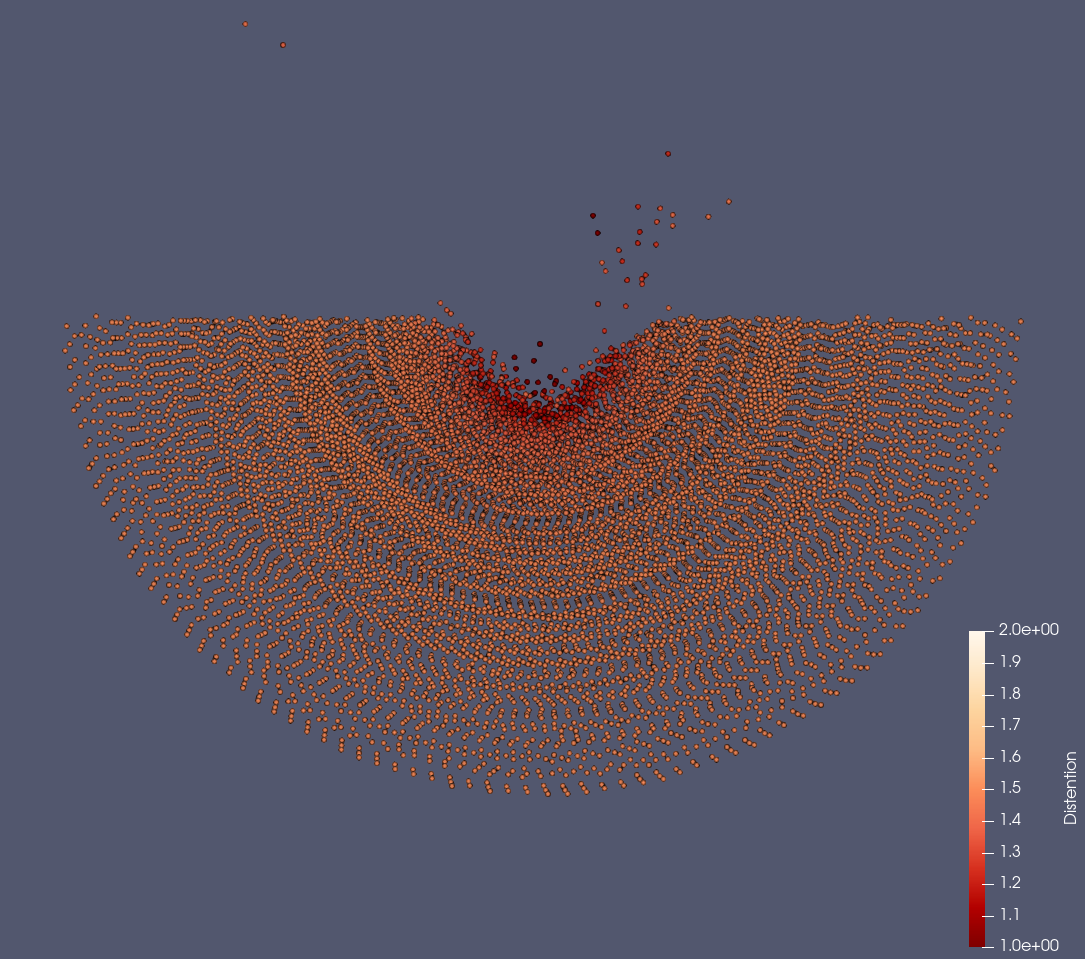
\includegraphics[keepaspectratio,
				width=0.25\paperwidth,
				height=\paperheight]{crater_por33_str1e4.png}};
	\end{tikzpicture}
	\begin{tikzpicture}[remember picture,overlay]
		\node[xshift=4.5cm,yshift=2.5cm] at (current page.south) {
			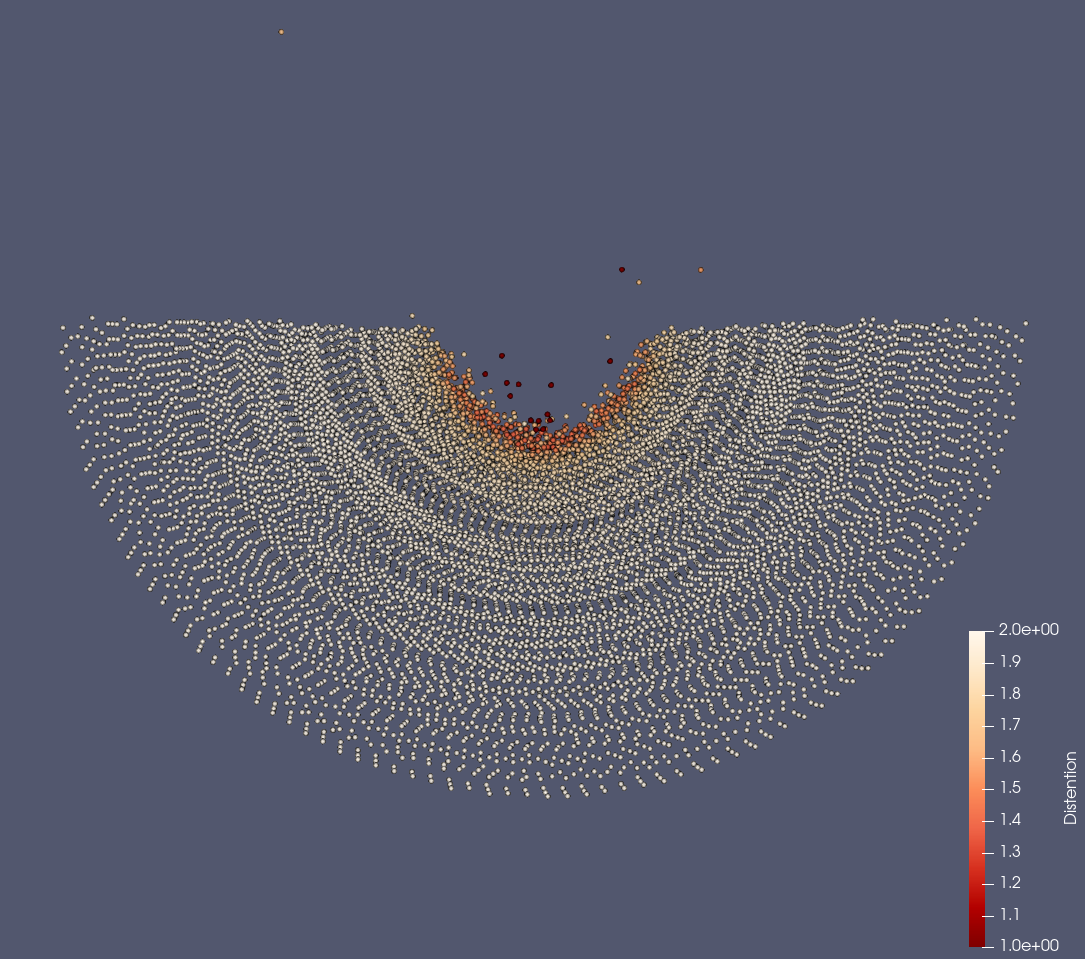
\includegraphics[keepaspectratio,
				width=0.25\paperwidth,
				height=\paperheight]{crater_por50_str1e3.png}};
	\end{tikzpicture}
\end{frame}

\begin{frame}{Personal observations about SPH}
	\begin{itemize}[<+->]
		\item A lot of individual physics implementable
		\item Interaction between physical models within a code can get complex
		\item Many different codes available
		\item Difficult to reproduce and compare results between different codes
		\item Dart setup could be useful as benchmark for solid models
	\end{itemize}
\end{frame}

\begin{frame}{Sources and additional information}
	Illustrations taken from Dart and Hera websites:
	\begin{itemize}
		\item https://dart.jhuapl.edu/
		\item https://www.nasa.gov/planetarydefense/dart
		\item https://www.esa.int/Safety\_Security/Hera
	\end{itemize}
	Papers:
	\begin{itemize}
		\item "Modeling impact outcomes for the Double Asteroid Redirection Test (DART) mission", Stickle et al., Procedia Engineering 2017
		\item "The role of asteroid strength, porosity and internal friction in impact momentum transfer", Raducan et al., Icarus 2019
	\end{itemize}
\end{frame}

\end{document}